\documentclass{article}
\usepackage[utf8]{inputenc}

\title{Foc Fault Report}
\author{hakan saraç}
\date{April 2020}

\usepackage{natbib}
\usepackage{graphicx}
\usepackage{indentfirst}
\usepackage{siunitx}
\usepackage{svg}


\addtolength{\oddsidemargin}{-.875in}
\addtolength{\evensidemargin}{-.875in}
\addtolength{\textwidth}{1.75in}
\addtolength{\topmargin}{-.875in}
\addtolength{\textheight}{1.75in}    
\begin{document}

\maketitle

\section{Introduction}
In this report, a field oriented control will be examined for open fault conditions

\section{Resistive Load} 
In this section, the model is constructed for a three phase voltage source system and a resistive load. The main objective is to observe the behaviour of the d-q variables under faulty conditions. To match the position of voltages and current, the load chosen to be a resistive load. The obtained results are listed in this section.



Properties of the simulated system is as follows:
\begin{itemize}
    \item Resistive Load (1 Ohm)
    \item Three phase voltage source 400Vpeak 50hz 
    \item The position is fixed to $2 \pi f t$
\end{itemize}


The purpose of this simulations is to observe the dynamics of dq transformation under faulty condition. Moreover, these simulations can provide information about a motor with multi three phase configuration. The fixed position can be inferred as one of the modules of the IMMD is faulted and other modules keeps the motor rotating. The analysis provides the aspect of the faulty module. \newline

The transformation equations are as follows:

\begin{equation}  \label{eq:eqnVd}
 v_d = \frac{2}{3}\Bigg(sin(\theta)*V_a + sin(\theta-\frac{2\pi}{3})*V_b + sin(\theta+\frac{2\pi}{3})*V_c\Bigg)
\end{equation}
\begin{equation} \label{eq:eqnVq}
v_q = \frac{2}{3}\Bigg(cos(\theta)*V_a + cos(\theta-\frac{2\pi}{3})*V_b + cos(\theta+\frac{2\pi}{3})*V_c\Bigg)
\end{equation}
\begin{equation} \label{eq:eqnV0}
 v_0 = \frac{2}{3}\Bigg(\frac{1}{2}V_a+\frac{1}{2}V_b+\frac{1}{2}V_c\Bigg)
\end{equation}
\subsection{Simulation Properties}
The simulation run for 2 seconds. When time equals to 1 second, a resistance value of $5e11$  ohm is added to phase a, in order to simulated an open phase fault.

\subsection{Simulation Results}
The simulation results are provided in Figure \ref{fig:ResistiveLoad_Vabc}, \ref{fig:ResistiveLoad_Iabc}, \ref{fig:ResistiveLoad_Vqd0}, \ref{fig:ResistiveLoad_Iqd0}. Since the current has to other return path, the current waveforms turn out to be 180 degrees apart of each other. 

When the fault occurs, the magnitude of the voltages changes to $346.41$ according to the simulation results. This change is due to the fact that the \textbf{load resistance doubles} and the voltage accross the resistances become \textbf{line to line voltage}. 
The analytical derivation of the faulty voltage waveforms are as follows. 


At t=1 $V_a$ voltage becomes zero, assume that at time $V_b$ and $V_c$ voltages are $sin(\theta)$ and $-sin(\theta)$ respectively. The equation \ref{eq:eqnVd}, \ref{eq:eqnVq},  \ref{eq:eqnV0} becomes \ref{eq:eqnVd_1}, \ref{eq:eqnVq_1},  \ref{eq:eqnV0_1} respectively:
\begin{equation} \label{eq:eqnVd_1}
    v_d = \frac{2}{3}\Bigg(sin(\theta)sin(\theta-\frac{2\pi}{3}) - sin(\theta)sin(\theta+\frac{2\pi}{3})\Bigg) =  -\frac{2}{3}\Bigg(sin(2\theta)sin(\frac{2\pi}{3})\Bigg)
\end{equation}
\begin{equation} \label{eq:eqnVq_1}
v_q = \frac{2}{3}\Bigg(sin(\theta)cos(\theta-\frac{2\pi}{3}) - sin(\theta)cos(\theta+\frac{2\pi}{3})\Bigg) =  \frac{2}{3}\Bigg(cos(2\theta)sin(-\frac{2\pi}{3})+sin(\frac{2\pi}{3})\Bigg)
\end{equation}
\begin{equation} \label{eq:eqnV0_1}
 v_0 = \frac{2}{3}(\frac{1}{2}sin(\theta)-\frac{1}{2}sin(\theta)) = 0
\end{equation}

It can be seen that the iq current and id currents are oscillating at frequency 100 Hz (see Figure \ref{fig:ResistiveLoad_Vqd0} and \ref{fig:ResistiveLoad_Iqd0}). The q component has a DC component as can be seen from Eqn. \ref{eq:eqnVq_1}. This DC component value states that under faulty conditions, this phase configuration can produce torque. However, since the d component is not zero anymore, it can cause saturation and/or demagnetization. This point should be taken into consideration when applying FOC. The simulation model is provided in \ref{fig:ModelResistive}.

\begin{figure}[h!]
\centering
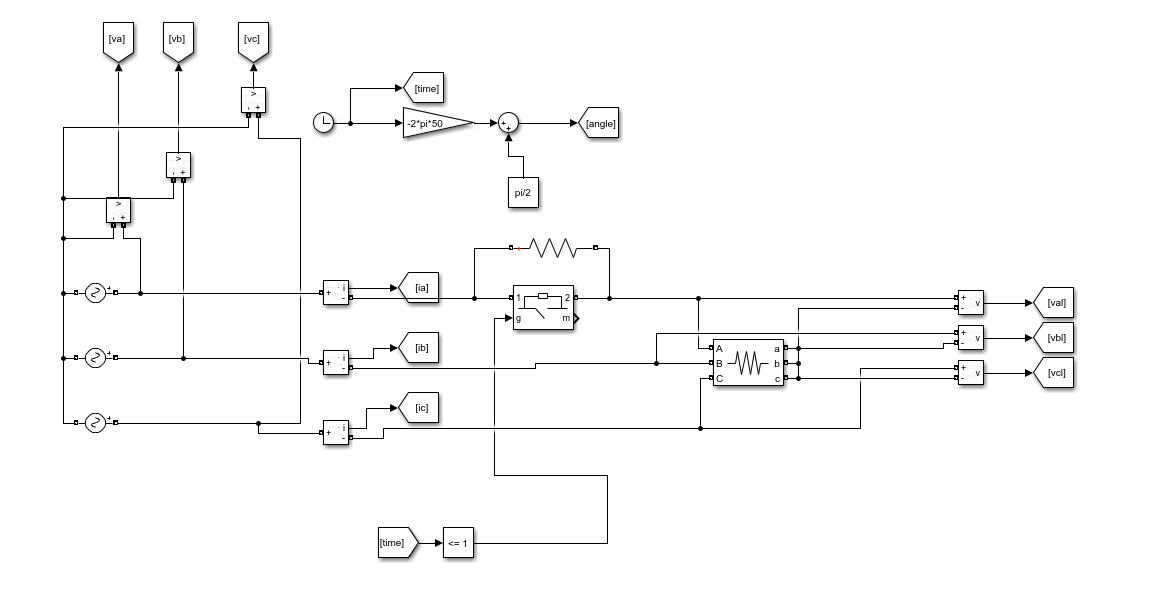
\includegraphics[scale=0.35]{Figures/ResistiveLoad/Model.PNG}
\caption{Voltage waveforms }
\label{fig:ModelResistive}
\end{figure}

\begin{figure}[h!]
\centering
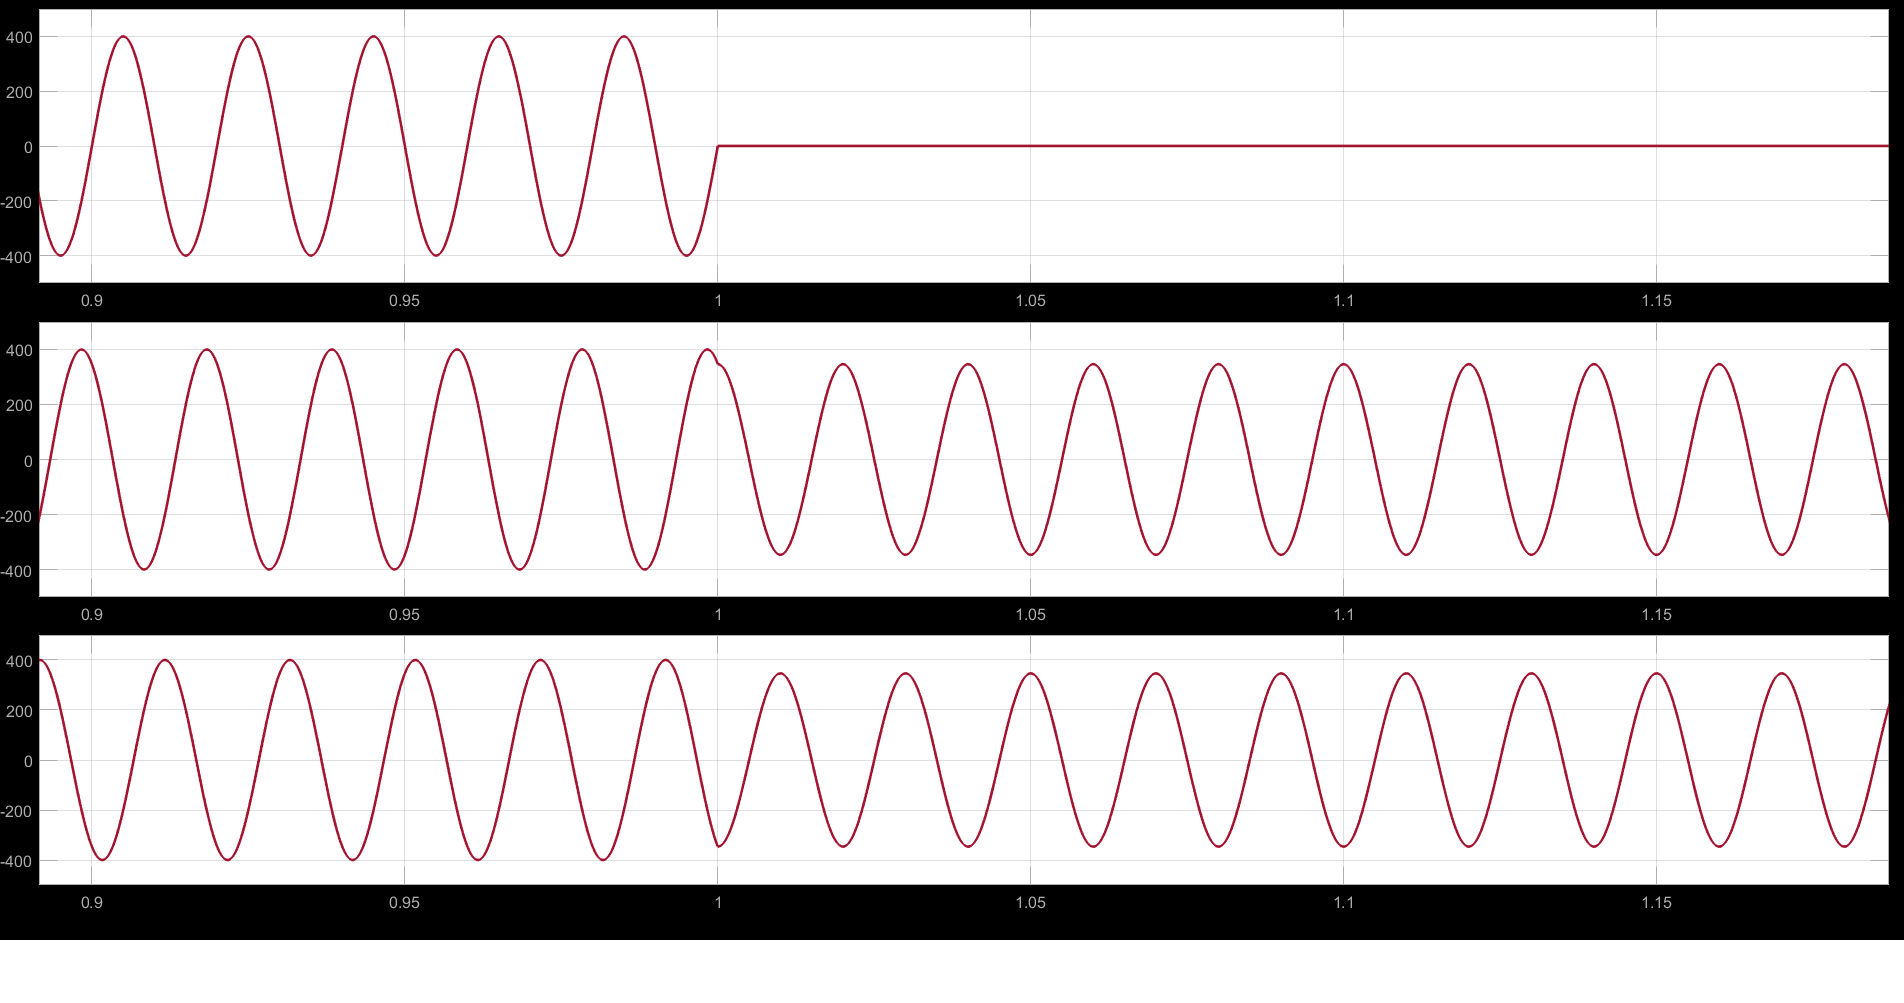
\includegraphics[scale=0.35]{Figures/ResistiveLoad/Vabc.png}
\caption{Voltage waveforms }
\label{fig:ResistiveLoad_Vabc}
\end{figure}

\begin{figure}[h!]
\centering
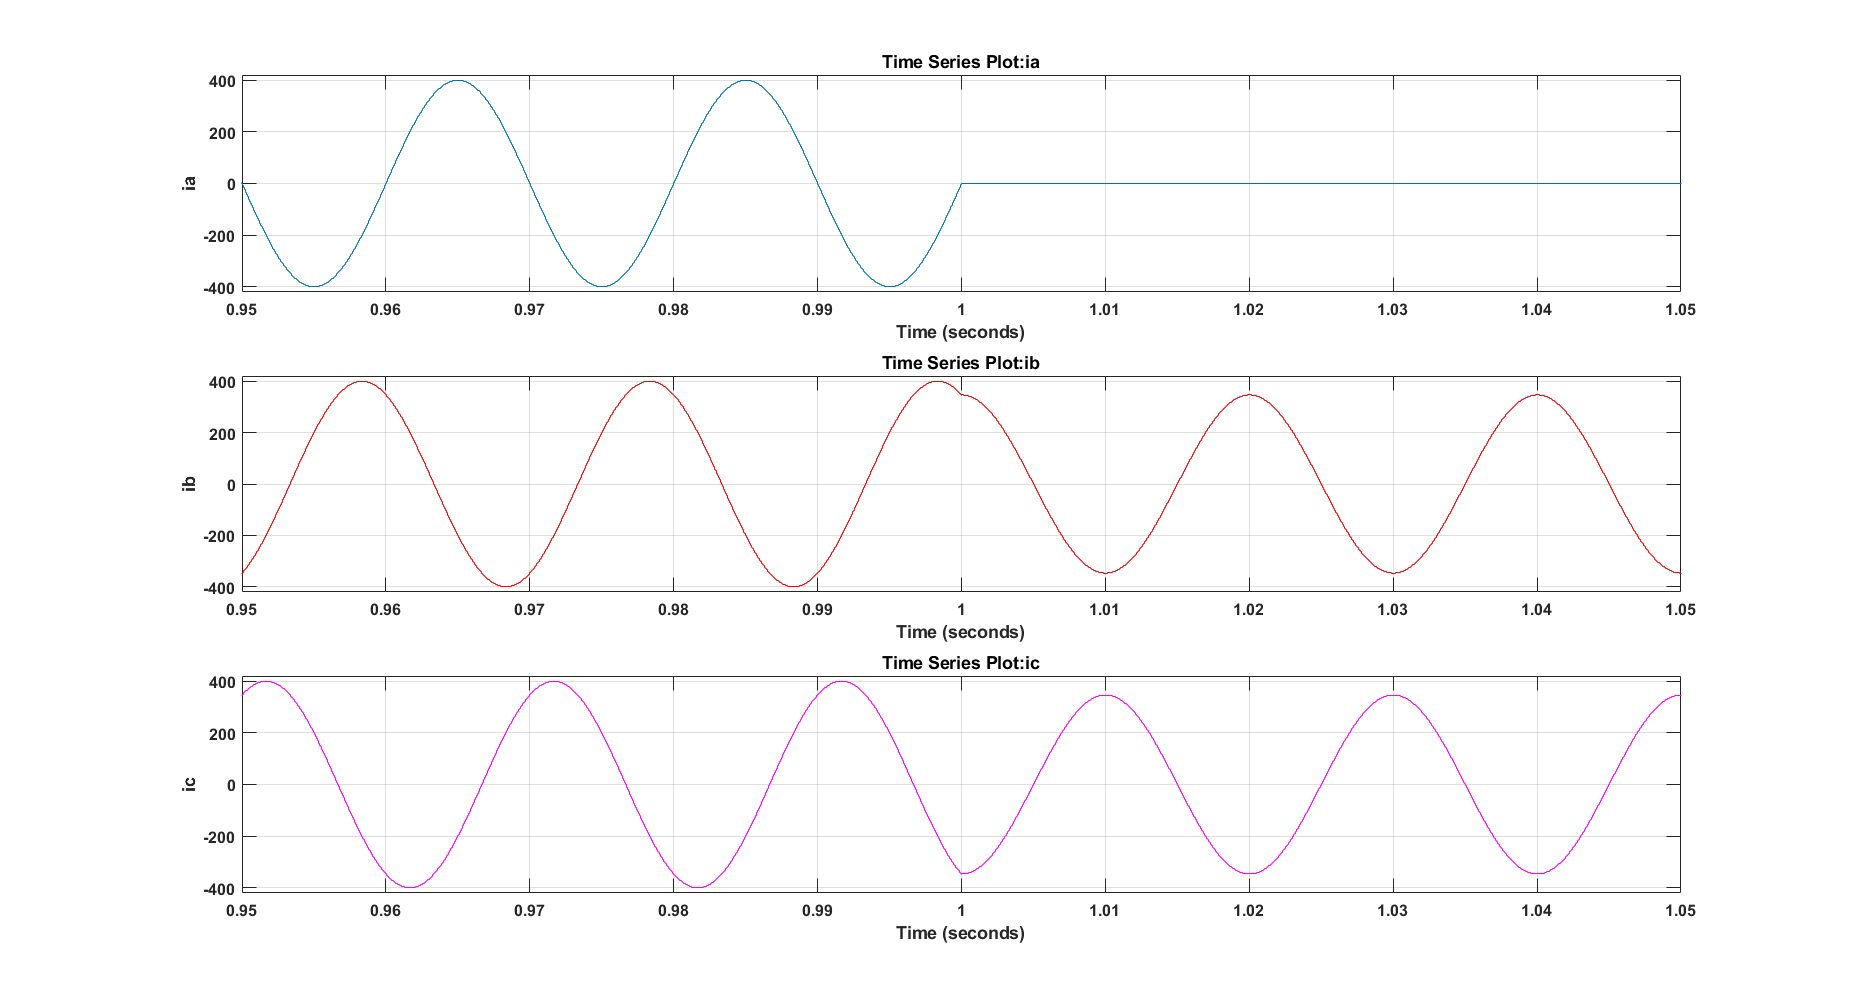
\includegraphics[scale=0.35]{Figures/ResistiveLoad/Iabc.png}
\caption{Current waveforms}
\label{fig:ResistiveLoad_Iabc}
\end{figure}

\begin{figure}[h!]
\centering
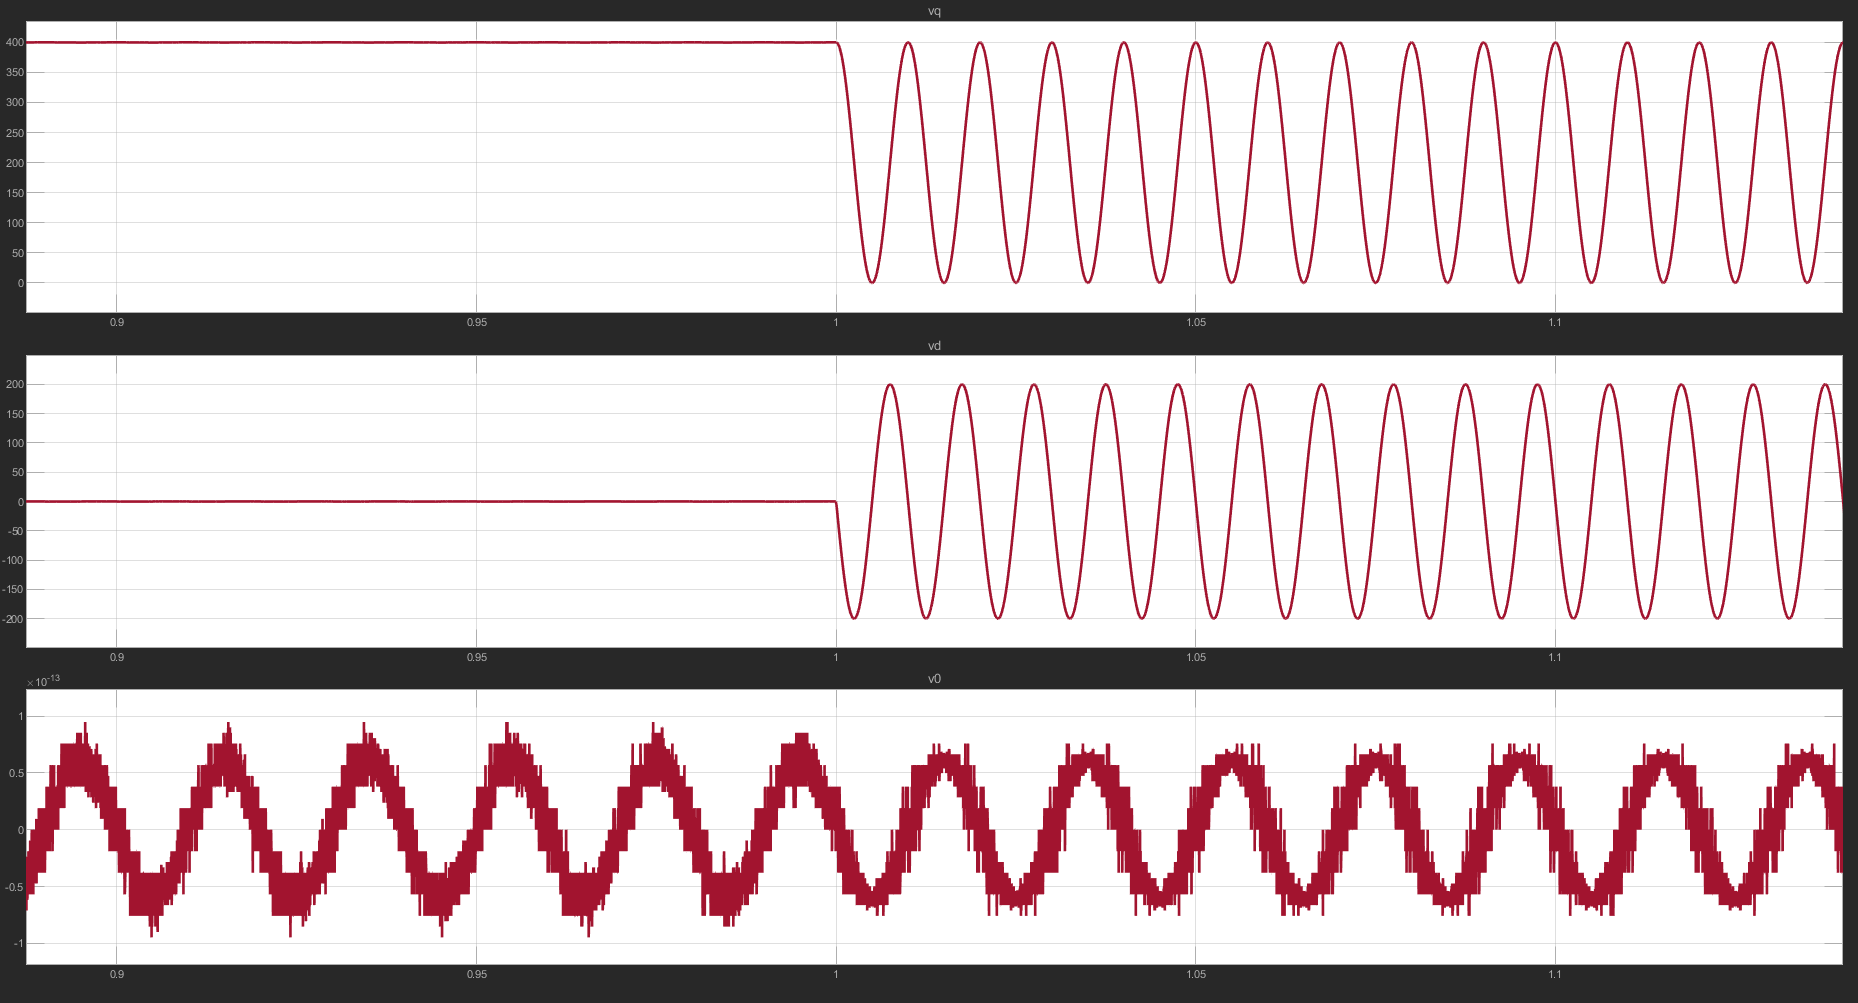
\includegraphics[scale=0.35]{Figures/ResistiveLoad/Vqd0.png}
\caption{qd0 voltages}
\label{fig:ResistiveLoad_Vqd0}
\end{figure}


\begin{figure}[h!]
\centering
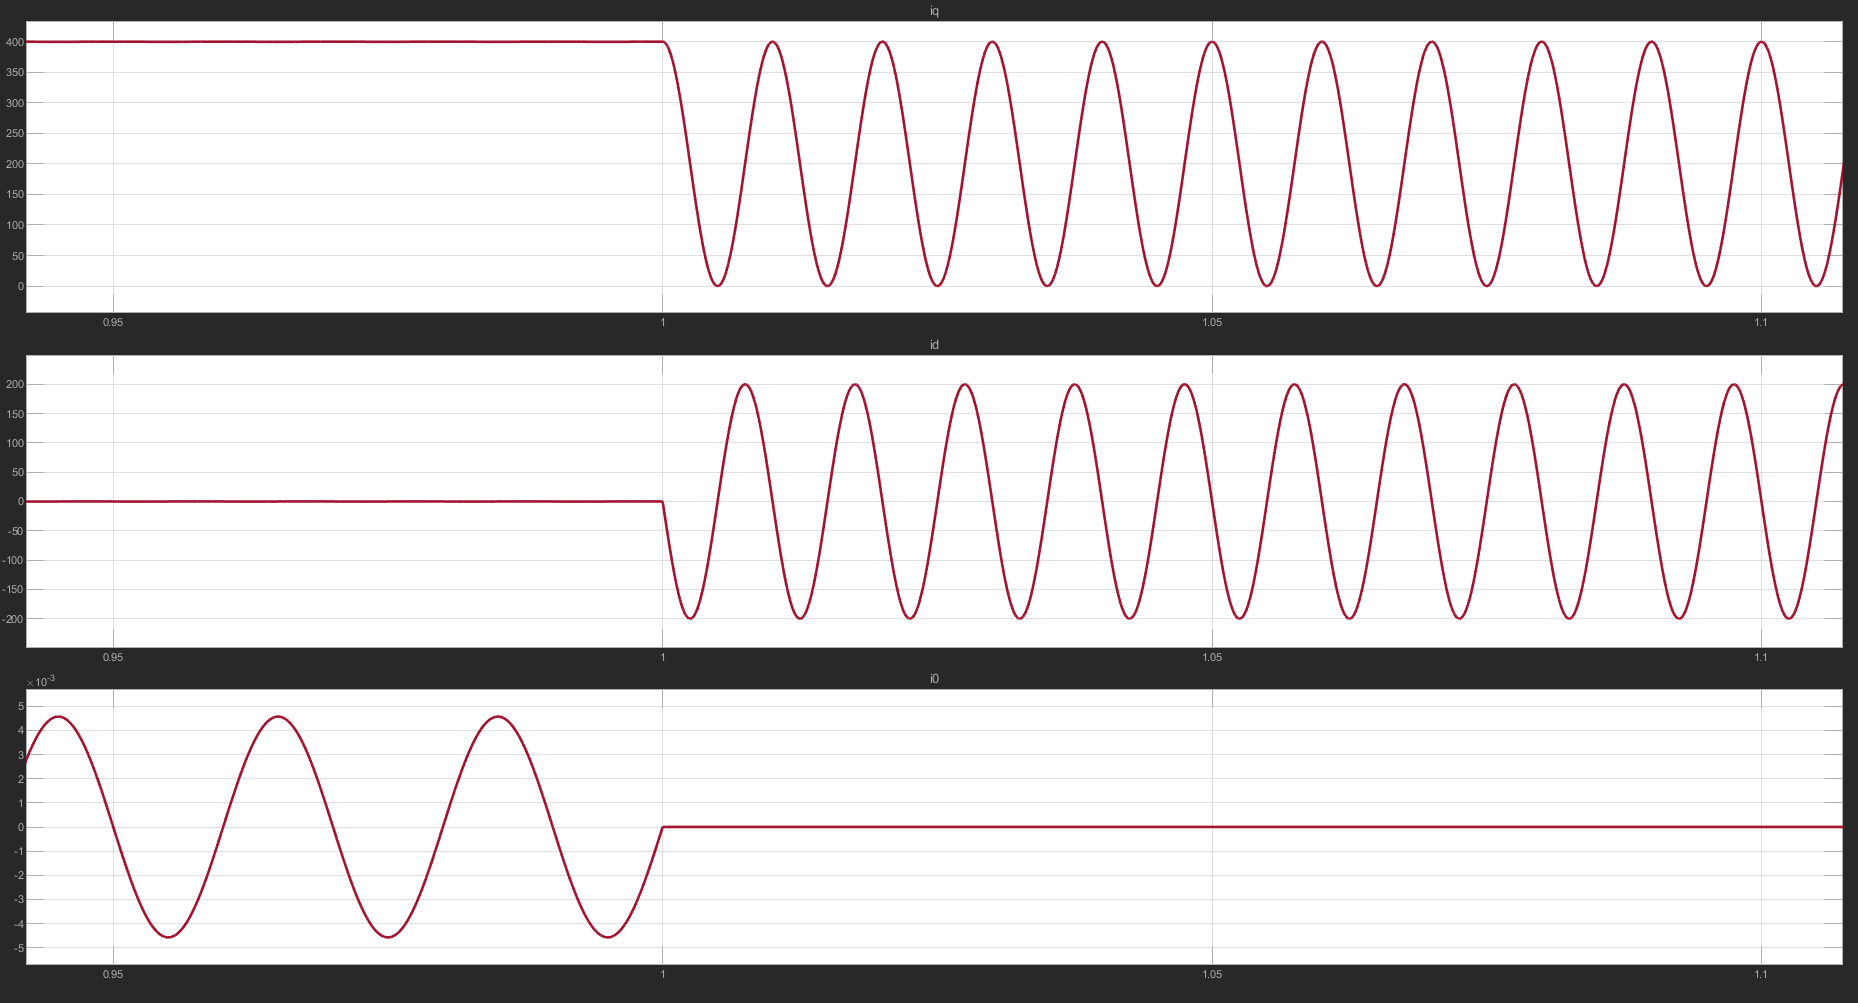
\includegraphics[scale=0.35]{Figures/ResistiveLoad/Iqd0.png}
\caption{qd0 currents}
\label{fig:ResistiveLoad_Iqd0}
\end{figure}


\section{Single Three Phase Motor Drive - One Phase Fault}
In this section, a three phase machine is simulated for an open phase fault, similar to the that of previous section. The speed of the machine is controlled using FOC. The simulation results are provided in Figures \ref{fig:fault_moment}, \ref{fig:ref_update_under_fault}, \ref{fig:overall_single}. Properties of the simulation as follows
\begin{itemize}
    \item Speed ref starts at 200 rpm and updated to 100 rpm at t=6sec
    \item Open phase fault (on phase A) occurs at t=3sec
    \item Load torque kept constant at 5Nm
\end{itemize}

It can be seen that the motor can continue its operation but with a very large torque pulsations. The variation of dq parameters can also contribute this issue since PI controller are not good at tracking time varying signals. There is considerable amount of d current, which can be dangerous as mentioned in previous section. 

The position reference is affected by the generated torque as well.

\begin{figure}[h!]
\centering
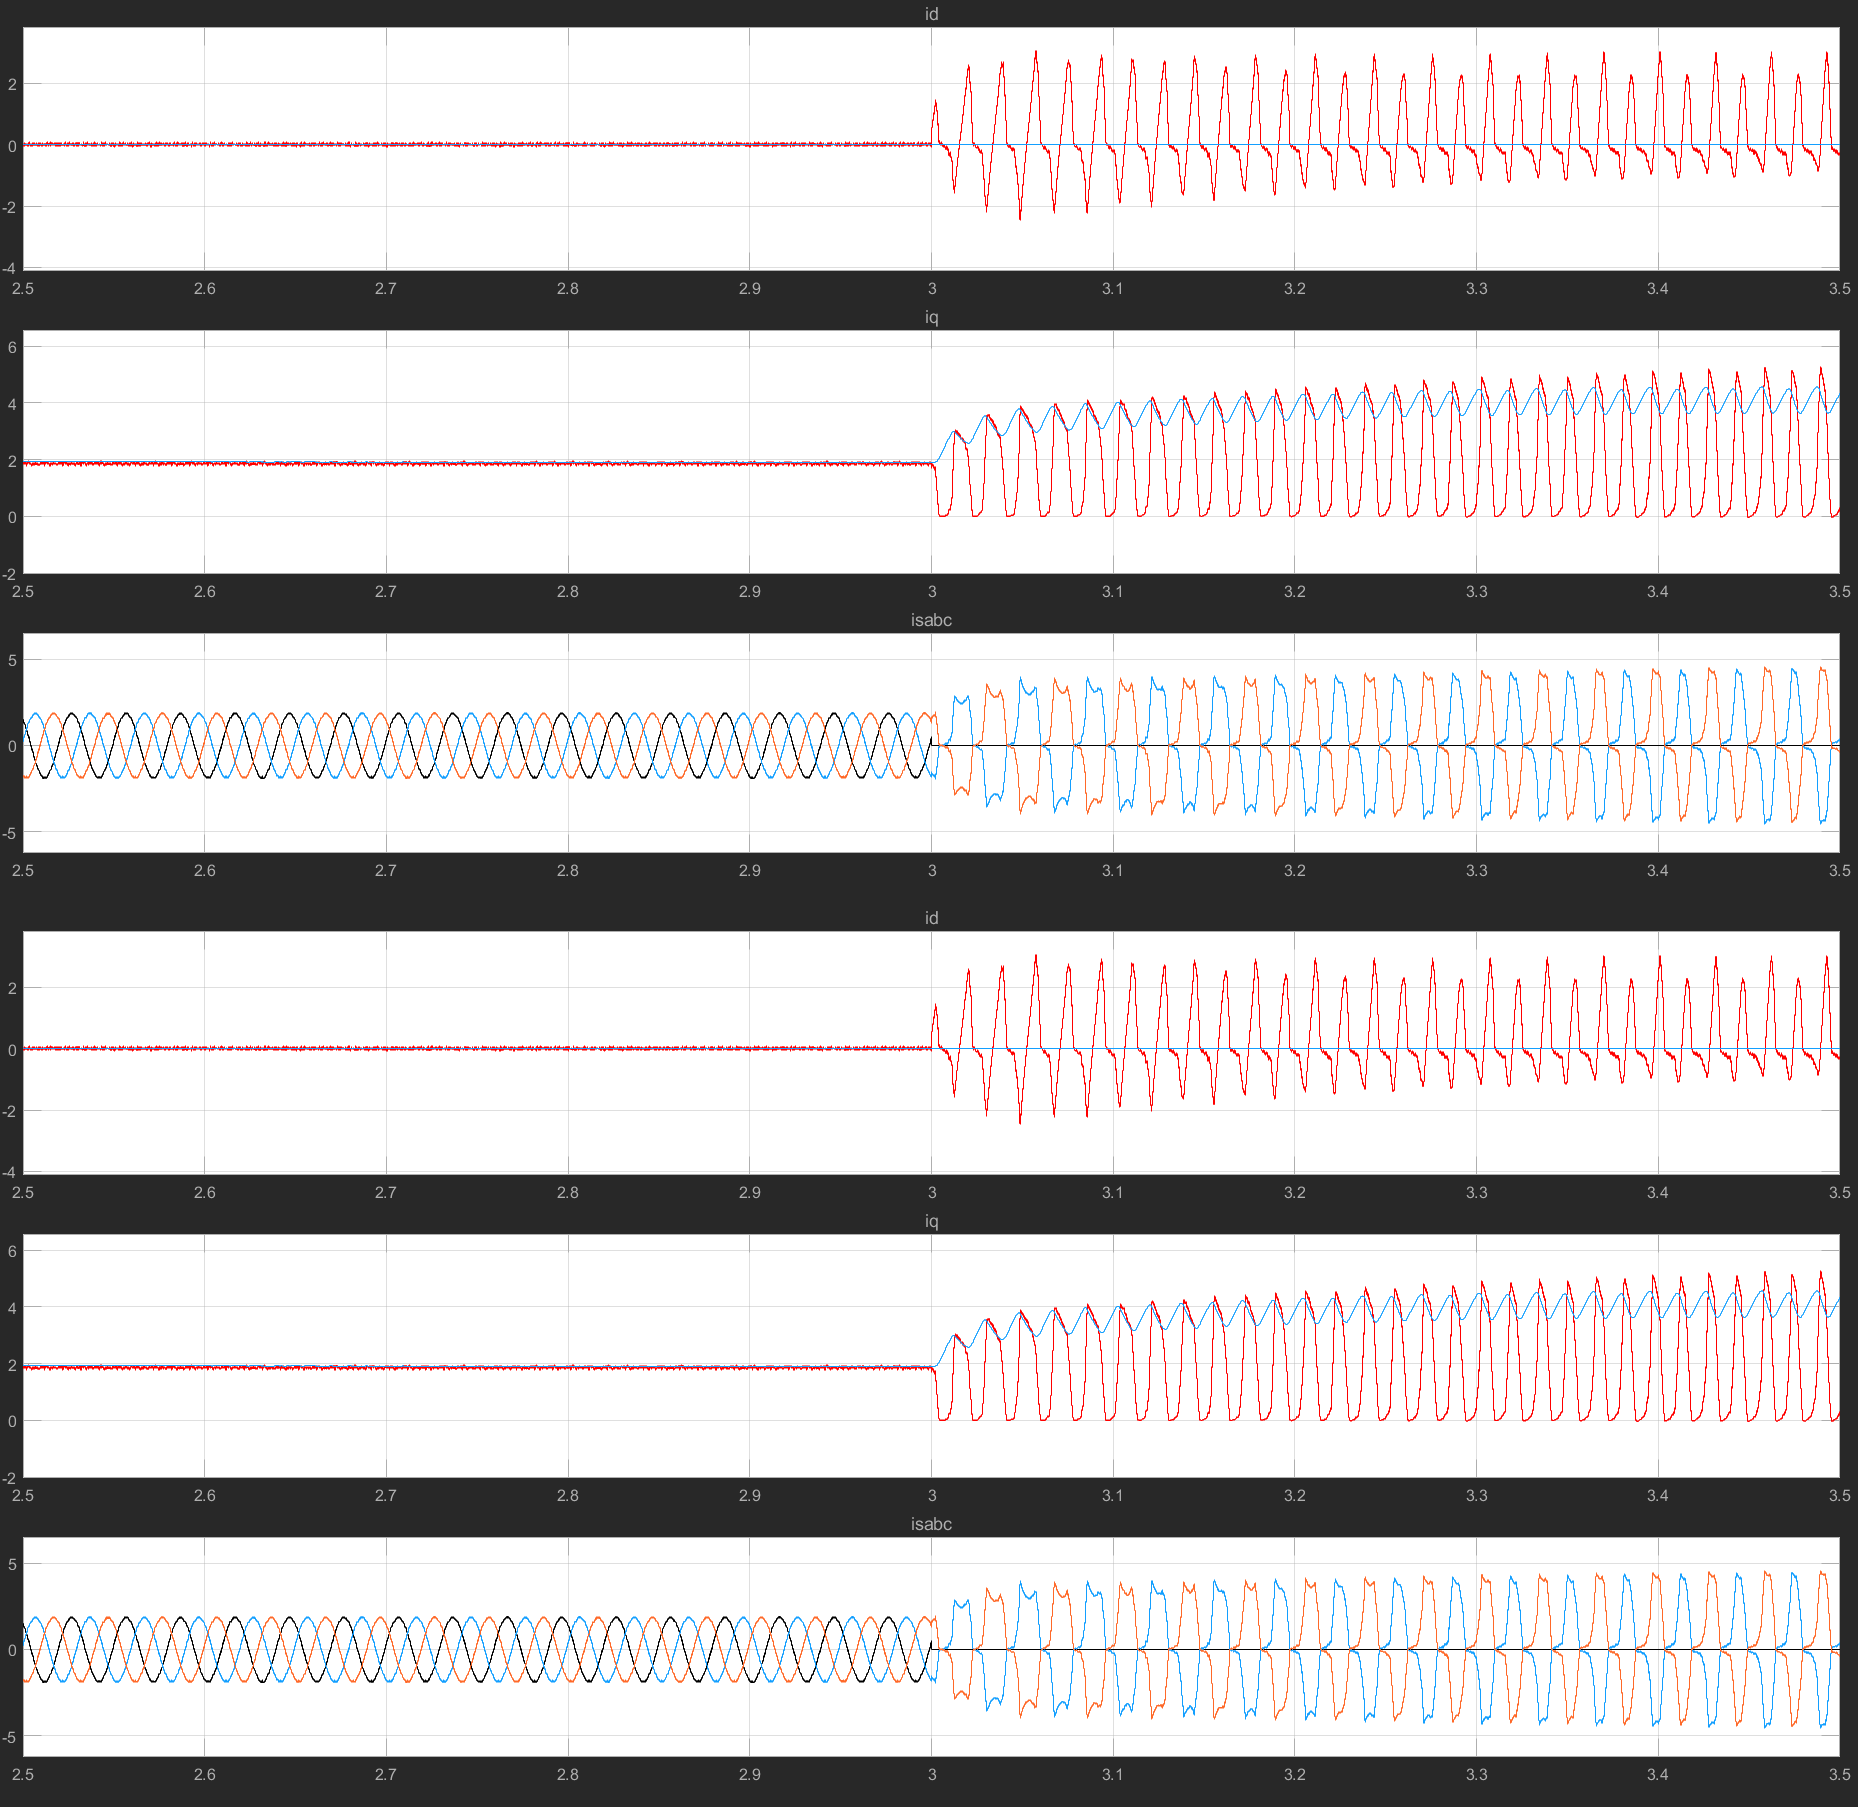
\includegraphics[scale=0.3]{Figures/SingleModule/FaultMoment.png}
\caption{Fault moment for single module}
\label{fig:fault_moment}
\end{figure}

\begin{figure}[h!]
\centering
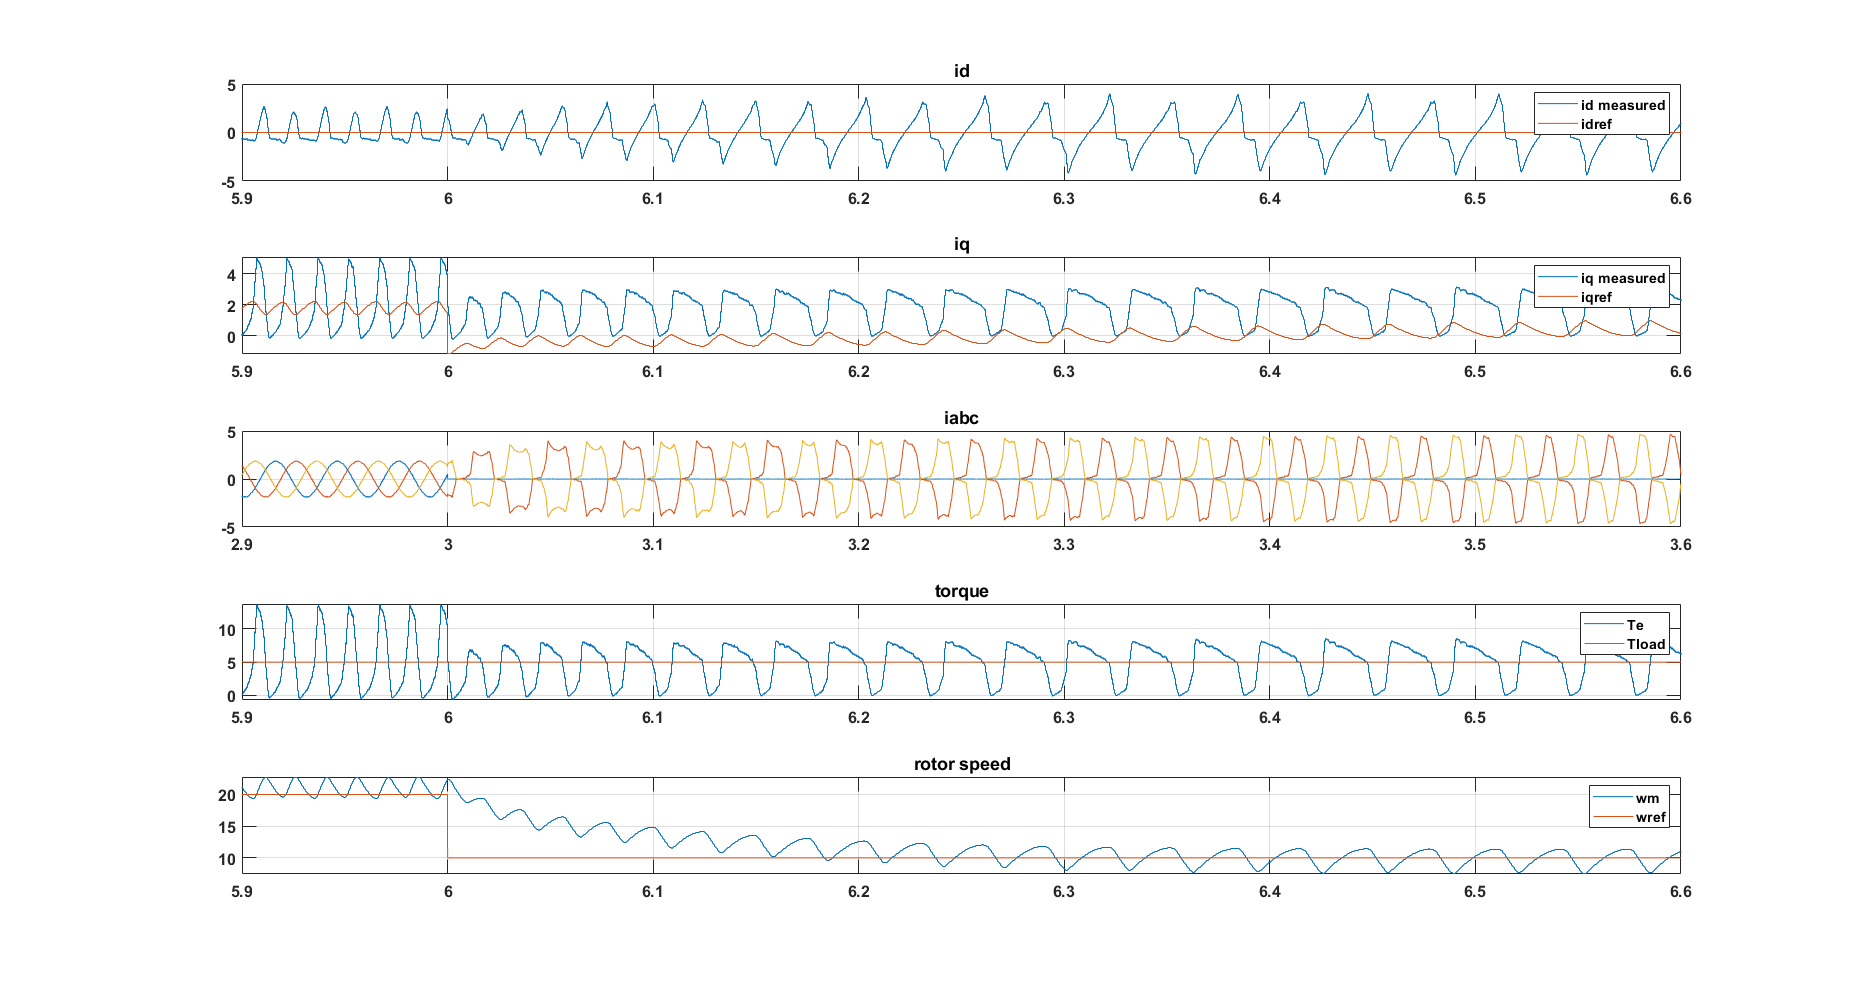
\includegraphics[scale=0.3]{Figures/SingleModule/SpeedRefUpdateUnderFault.png}
\caption{Speed reference update under fault}
\label{fig:ref_update_under_fault}
\end{figure}

\begin{figure}[h!]
\centering
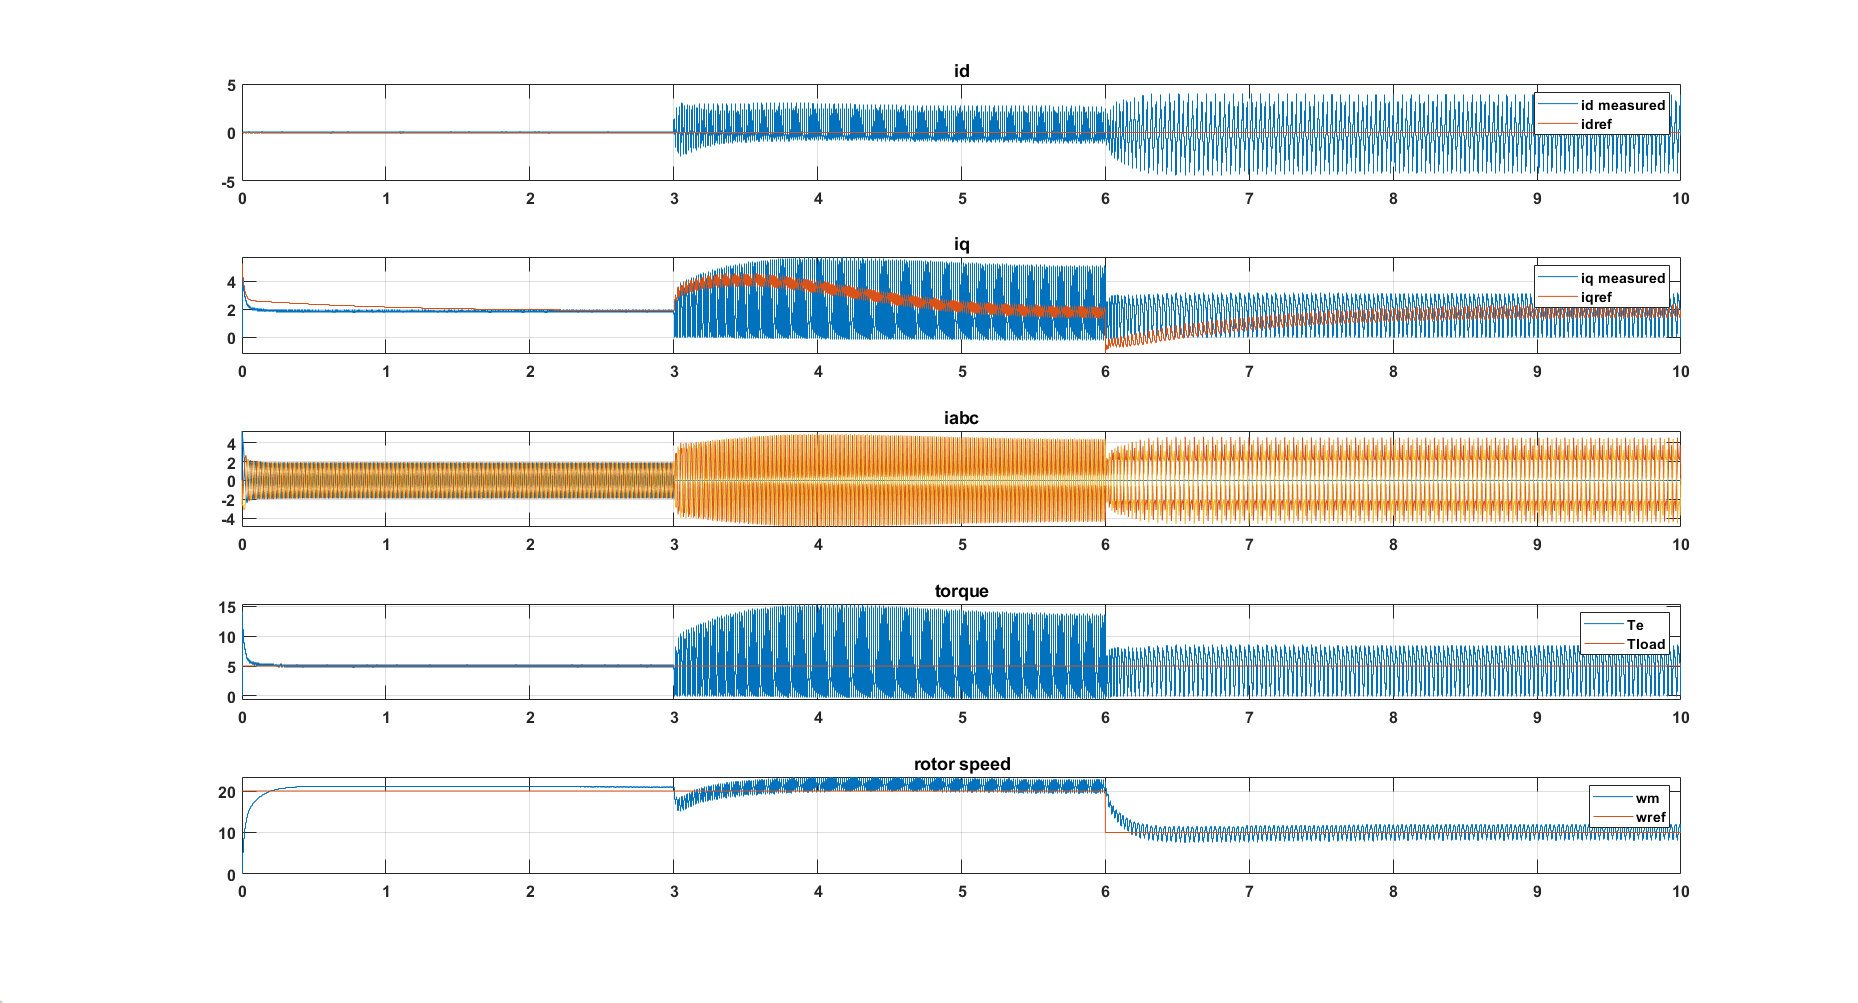
\includegraphics[scale=0.3]{Figures/SingleModule/Overall.png}
\caption{Overall single module simulation}
\label{fig:overall_single}
\end{figure}


\section{Dual Three Phase Motor Drive - One Phase Fault}
Simulation results are provided in Figure \ref{fig:overall_dual}. The simulation properties are as follows:

\begin{itemize}
    \item Speed ref starts at 200 rpm and updated to 100 rpm at t=6sec
    \item Open phase fault (on phase A of module 1)  occurs at t=3sec
    \item Load torque kept constant at 4Nm
\end{itemize}

The FOC tries to equalize the torque efforts of both modules. The module 2 seems to be not significantly affected by the fault occured on module 1 (discarding mutual coupling effects). Event though the system continues its operation, the id iq pulsations are significantly high and these phase groups can affect each other.

\begin{figure}[h!]
\centering
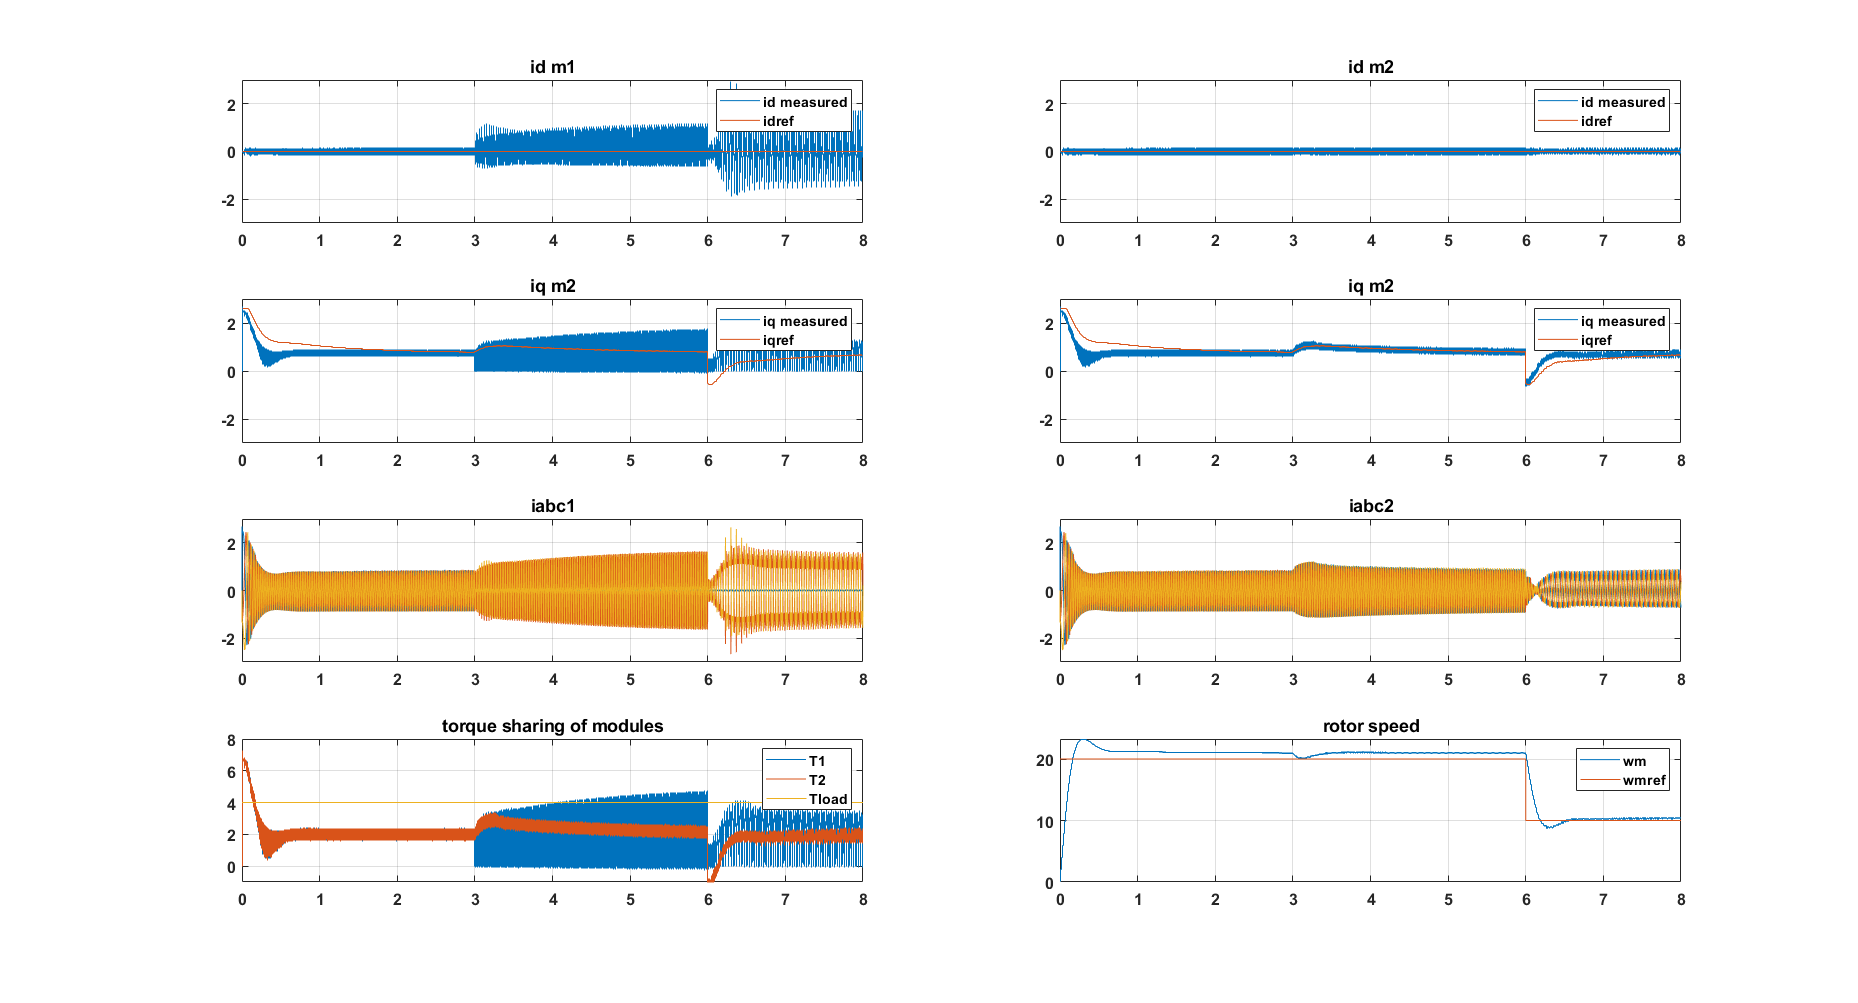
\includegraphics[scale=0.3]{Figures/DualModule/Overall.png}
\caption{Overall dual module simulation}
\label{fig:overall_dual}
\end{figure}

\subsection{Conclusion}

In this report it is observed that the machine with single module can continue its operation and generate torque. However, since a rotating MMF cannot be created, the generated torque has many ripples. 
In the dual module case, the second module is nearly unaffected. To reduce the torque ripple in the case of a fault, the healthy module can continue operation with a considerable contribution to torque from the faulty module.


\bibliographystyle{plain}
\end{document}
